%% Template for EU deliverable, using the deliverable.sty style file

\documentclass[12pt,a4paper,twoside]{article}

%% common package
\usepackage[headers]{deliverable}
\usepackage{xspace}
\usepackage{verbatim}
\usepackage[usenames]{color}
\usepackage{listings}
%\usepackage[usenames,dvipsnames,table]{xcolor}
\usepackage[pdftex,dvips]{graphicx}
\usepackage{url}
\usepackage{array}
%%

%%insert here other packages needed by sections

%%

%%%%%%%%%%%%%%%%%%%%%%%%%%%%%%%%%%%%%%%%%%%%%%%%%%%%%%%%%%%%%%%%%%%%%%%%%%%%%%
%%% Titlepage
%%%%%%%%%%%%%%%%%%%%%%%%%%%%%%%%%%%%%%%%%%%%%%%%%%%%%%%%%%%%%%%%%%%%%%%%%%%%%%

% declaration of variables used in style
\deliverableDocnumber{D3.3}
\deliverableTitle{Local solver in compliant and unforeseen cases}
\deliverableAuthor{Vincent Padois$^{1}$}
\deliverableResponsiblePartner{UPMC}
\deliverableAffiliation{% Insert here authors affiliations
 $^1$ Sorbonne Universit\'es, UPMC Paris 06, UMR CNRS 7222, Institut des Syst\`emes Intelligents et de Robotique (ISIR), F-75005, Paris, France.
 }


\deliverableCoordinator{Vincent Padois}
\deliverableActivityNumber{n} %% n=1,..,10
\deliverableActivity{Local solver in compliant and unforeseen cases}
\deliverableDoctype{Deliverable} %% or Prototype
\deliverableClassification{Public} % or Consortium
\deliverableDistribution{Consortium} %
\deliverableStatus{Final} % Draft or Final
\deliverableDeliveryDate{28/2/2017}
\deliverableFile{D3.3.pdf} % please do not use "-" in the name
\deliverableVersion{1.0}
\deliverableDate{Feb.~28, 2017}
\deliverableYear{2017}
\deliverablePages{\pageref{LastPage}}
\deliverableChangelog{}
\deliverableProjectStartingDate{1st March 2013}
\deliverableProjectEndDate{28th February 2017}
\deliverableProjectAcronym{CoDyCo}
\deliverableProjectTitle{Whole-Body Compliant Dynamical Contacts in Cognitive Humanoids}
\deliverableContractNumber{600716}
\deliverableProjectCoordinator{Istituto Italiano di Tecnologia}
\deliverableProjectUrl{www.codyco.eu}
\deliverableFrameworkProgramme{FP7}
 
\deliverableWorkpackage{WP3}
\deliverableEditors{Vincent Padois}
\deliverableContributors{Ryan Lober, Francesco Nori, Vincent Padois, Daniele Pucci, Francesco Romano, Olivier Sigaud, Silvio Traversaro}


\deliverableAbstract{Highly redundant robots, such as humanoids, can execute multiple simultaneous tasks allowing them to perform complex whole-body behaviors. Unfortunately, tasks are generally planned without close consideration for the underlying controller being used, or the other tasks being executed. Because of this, tasks are often incompatible with one another and/or the system constraints, and cannot always be accomplished simultaneously. These incompatibilities can be managed using prioritization and gains, but tuning them is tedious.
After introducing a passivity based control approach designed to maximally benefit from a potential external support in a multi-contact interaction (here  a standing motion using external support), %recalling the structure of the whole-body controller that will be used for the final year demonstration (based on the generic controller architecture presented in Deliverables~3.2~\cite{deliverable32} and 5.3~\cite{deliverable53}), 
this deliverable introduces and develops the concept of task compatibility optimization, as a alternative/complementary method to the prioritization learning methods introduced in Deliverable~4.3~\cite{deliverable43}. Task compatibility optimization automatically improves task compatibility by modifying their trajectories using reinforcement learning. To do so, the tasks are iteratively optimized by minimizing a compatibility cost, which measures the compatibility between one or more tasks, and the system constraints. Using two common, CoDyCo related, scenarios, it is shown that that task compatibility optimization results in whole-body behaviors which better match the original intent of the task combination without the need for manual tuning of task/controller parameters, heuristics, or re-planning.}
\deliverableReviewers{}
\deliverableKeywordList{Whole-body controllers,  Multi-contacts, Unforseen situations, Task compatibility optimization, Learning and adaptation}

%%%%%%%%%%%%%%%%%%%%%%%%%%%%%%%%%%%%%%%%%%%%%%%%%%%%%%%%%%%%%%%%%%%%%%%%%%%%%%
%%% Sections
%%%%%%%%%%%%%%%%%%%%%%%%%%%%%%%%%%%%%%%%%%%%%%%%%%%%%%%%%%%%%%%%%%%%%%%%%%%%%%

%% constants
\newcommand{\botegoCaps}{BOTEGO}
\newcommand{\certhCaps}{CERTH}
\newcommand{\cybionCaps}{CYBION}
\newcommand{\nuigCaps}{NUIG}
\newcommand{\ubitechCaps}{UBITECH}
%%

%%%%%%%%%%%%%%%%%%%%%%%%%%%%%%%%%%%%%%%%%%%%%%%%%%%%%%%%%%%%%%%%%%%%%%%%%%%%%%
%%% Misc. by Vincent
%%%%%%%%%%%%%%%%%%%%%%%%%%%%%%%%%%%%%%%%%%%%%%%%%%%%%%%%%%%%%%%%%%%%%%%%%%%%%%
\usepackage{titlesec}
\newcommand{\sectionbreak}{}
\graphicspath{{./figure/}}
\usepackage{pdfpages}
%\usepackage{caption}
%\usepackage{subcaption}
%\usepackage{caption}
%\usepackage{subcaption}
\usepackage{slashbox}
\usepackage{multirow}
\usepackage{appendix}
\usepackage{amsmath} % assumes amsmath package installed
\usepackage{amssymb}  % assumes amsmath package installed
%\usepackage[ruled,vlined,linesnumbered]{algorithm2e}
\usepackage{mathtools}
\usepackage{graphicx}
\usepackage{hyperref}
\hypersetup{
    %bookmarks=true,         % show bookmarks bar?
    unicode=false,          % non-Latin characters in Acrobat’s bookmarks
    pdftoolbar=true,        % show Acrobat’s toolbar?
    pdfmenubar=true,        % show Acrobat’s menu?
    pdffitwindow=false,     % window fit to page when opened
    pdfstartview={FitH},    % fits the width of the page to the window
    pdftitle={D33.pdf},    % title
    pdfauthor={Vincent Padois},     % author
    pdfsubject={Local solver in compliant and unforeseen cases},   % subject of the document
    pdfcreator={Vincent Padois},   % creator of the document
    pdfproducer={Vincent Padois}, % producer of the document
    pdfkeywords= {Whole-body controllers,  Multi-contacts, Non-rigid contacts and unforseen situations, Learning and adaptation}, % list of keywords
    pdfnewwindow=true,      % links in new window
    colorlinks=true,       % false: boxed links; true: colored links
    linkcolor=black,          % color of internal links (change box color with linkbordercolor)
    citecolor=black,        % color of links to bibliography
    filecolor=black,      % color of file links
    urlcolor=black           % color of external links
}

\newcommand{\vect}[1]{\mbox{\boldmath${#1}$}}%$
\newcommand{\av}{\vect{\chi}}
\newcommand{\tens}[1]{#1}
%\DeclareMathOperator*{\argmin}{argmin}

%--------------------------------------------------------%
%						PACKAGES							%
%--------------------------------------------------------%

\usepackage{amsmath} % assumes amsmath package installed
\usepackage{amsfonts}
\usepackage{amssymb}  % assumes amsmath package installed

\usepackage[pdftex]{graphicx} %demo during testing
\graphicspath{{images/}}
\usepackage{float}
\usepackage[caption=true]{subfig}
\usepackage[font=small]{caption}

\usepackage{IEEEtrantools}
\usepackage{mathtools}



% \usepackage{pdfsync} % to be able to click a pdf and move to the corresponding latex location compile with: pdflatex [file_name] -synctex=1

\usepackage{algorithm}
\usepackage{algorithmicx}
\usepackage{algpseudocode}
\algdef{SE}[DOWHILE]{Do}{doWhile}{\algorithmicdo}[1]{\algorithmicwhile\ #1}%

%
% \usepackage[labelformat=simple]{subcaption}
% \renewcommand\thesubfigure{(\alph{subfigure})}
%
\usepackage[percent]{overpic}
% \usepackage{showframe}
%\usepackage{pdflscape}

\usepackage{textcomp}
\usepackage[table,xcdraw]{xcolor}






\usepackage{tikz}
\usetikzlibrary{shapes,arrows,positioning,fit}
\pgfdeclarelayer{background}
\pgfsetlayers{background,main}
\definecolor{optim_color}{RGB}{49,30,189}
\tikzset{
    %Define standard arrow tip
    %Define style for boxes
    >=stealth',
    punkt/.style={
           rectangle,
           rounded corners,
           draw=black, very thick,
           text width=10em,
           minimum height=2em,
           text centered},
    optim_box/.style={
           rectangle,
           rounded corners,
           fill=optim_color!5,
           draw=optim_color, very thick,
           text width=8em,
           minimum height=2em,
           text centered},
    % Define arrow style
    pil/.style={
            >=stealth',
           ->,
           thick,
           shorten <=2pt,
           shorten >=2pt,},
    optim_pil/.style={
            >=stealth',
           ->,
           draw=optim_color, thick,
           shorten <=2pt,
           shorten >=2pt,}
}









\newcommand{\var}{\sigma^{2}}
\newcommand{\bs}[1]{\boldsymbol{#1}}
\newcommand{\err}{\bs{\epsilon}}
\newcommand{\errd}{\dot{\err}}
\newcommand{\errdd}{\ddot{\err}}

\newcommand{\way}{\bs{\lambda}}


\DeclareMathOperator*{\argmin}{argmin}
%\newcommand{\acc}{\bs{\xi}^{*}_{i}}
% GTC = General Traj Coordinate Variable
\newcommand{\gtcs}{\xi}
\newcommand{\gtc}{\bs{\gtcs}}
\newcommand{\gtcd}{\dot{\gtc}}
\newcommand{\gtcdd}{\ddot{\gtc}}

% JSR = Joint Space Representation
\newcommand{\jsrs}{\nu}
\newcommand{\jsr}{\bs{\jsrs}}
\newcommand{\jsrd}{\dot{\jsr}}
\newcommand{\jsrdd}{\ddot{\jsr}}



\newcommand{\q}{\bs{q}}
\newcommand{\qd}{\dot{\bs{q}}}
\newcommand{\qdd}{\ddot{\bs{q}}}



\newcommand{\x}{\bs{x}}
\newcommand{\xd}{\dot{\bs{x}}}
\newcommand{\xdd}{\ddot{\bs{x}}}
\newcommand{\X}{\mathbb{X}}
\newcommand{\accref}{\xdd^{ref}_{i}}
\newcommand{\acc}{\xdd_{i}}

\newcommand{\rc}{TBRC}

\newcommand{\y}{\bs{y}}
\newcommand{\yd}{\dot{\bs{y}}}
\newcommand{\ydd}{\ddot{\bs{y}}}

\newcommand{\os}{operational-space}
\newcommand{\Os}{Operational-space}

\newcommand{\js}{joint-space}
\newcommand{\Js}{Joint-space}

\newcommand{\N}{\mathcal{N}}
\newcommand{\R}{\mathbb{R}}
%\newcommand{\sr}[1]{\subref{#1}}

\newcommand{\blam}{\bs{\lambda}}
\newcommand{\tlam}{\bs{t}^{\lambda}}

\newcommand{\GP}{\mathcal{GP}}
\newcommand{\C}{\mathcal{C}}
\newcommand{\optVar}{\bs{\omega}}
\newcommand{\OptVar}{\Omega}

\newcommand{\f}{\bs{\text{f}}}
\newcommand{\fe}{\f_{e}}

% \renewcommand{\algorithmiccomment}[1]{\hfill  ~#1\normalsize}
\newcommand{\tc}{\ \text{,}}
\newcommand{\tp}{\ \text{.}}

\newcommand{\obj}{\bs{\theta}}
\newcommand{\Obj}{\Theta}


%%%%%%%%%%%%%%%%%%%%%%%%%%%%%% BEGIN DOCUMENT
\begin{document}

\deliverableMaketitle

%%TODO move to style
\newcolumntype{L}[1]{>{\raggedright\let\newline\\\arraybackslash\hspace{0pt}}m{#1}}
\newcolumntype{C}[1]{>{\centering\let\newline\\\arraybackslash\hspace{0pt}}m{#1}}
\newcolumntype{R}[1]{>{\raggedleft\let\newline\\\arraybackslash\hspace{0pt}}m{#1}}

\textbf{Document Revision History}
\begin{center}
\begin{tabular}{|C{2cm}|C{3cm}|C{5cm}|C{4cm}|}
\hline
\textbf{Version}&\textbf{Date}&\textbf{Description}&\textbf{Author}\\\hline
v.~1.0 & Feb.~28, 2017 & Final version & Vincent Padois \\ \hline
\end{tabular}
\end{center}
 
 \clearpage

\newpage
\renewcommand*\contentsname{Table of Contents}
\renewcommand*\listfigurename{Index of Figures}
\tableofcontents
\newpage
\listoffigures
\newpage

%%%%%%%%%%%%%%%%%%%%%%%% Start deliverable content here.


\paragraph{Foreword:} Research works performed within the framework of CoDyCo and that directly relate to this deliverable are cited as \underline{\bf [xx]}. These papers being available online, they are not provided in Appendix of this deliverable.

\section{Introduction}
Highly redundant robots, such as humanoids, can execute multiple simultaneous tasks allowing them to perform complex whole-body behaviors. Unfortunately, tasks are generally planned without close consideration for the underlying controller being used, or the other tasks being executed. Because of this, tasks are often incompatible with one another and/or the system constraints, and cannot always be accomplished simultaneously. These incompatibilities can be managed using prioritization and gains, but tuning them is tedious.\\

After introducing a passivity based control approach designed to maximally benefit from a potential external support in a multi-contact interaction (here  a standing motion using external support), %recalling the structure of the whole-body controller that will be used for the final year demonstration (based on the generic controller architecture presented in Deliverables~3.2~\cite{deliverable32} and 5.3~\cite{deliverable53}), 
this deliverable introduces and develops the concept of task compatibility optimization, as a alternative/complementary method to the prioritization learning methods introduced in Deliverable~4.3~\cite{deliverable43}. Task compatibility optimization automatically improves task compatibility by modifying their trajectories using reinforcement learning. To do so, the tasks are iteratively optimized by minimizing a compatibility cost, which measures the compatibility between one or more tasks, and the system constraints. Using two common, CoDyCo related, scenarios, it is shown that that task compatibility optimization results in whole-body behaviors which better match the original intent of the task combination without the need for manual tuning of task/controller parameters, heuristics, or re-planning.

\section{Dealing with unforeseen situations: the case of external support}
\label{sec:controller}

%\subsection{The controller for the first and second year validation scenario} 
\label{sec:firstSecondValid}
Although the above optimization can handle several control tasks, the control architecture we have been working on is composed of essentially two tasks.
\begin{figure}[t]
    \centering{
    % \includsvg{imgs/model}
        \def\svgwidth{0.2\columnwidth}         
        \includegraphics[width=0.65\columnwidth]{images/iCubInteractionOneFoot.jpg}
    \caption{A screen-shot of the one-foot balancing demo }
    \label{fig:oneFootBalnacing}
    }
\end{figure}

\begin{enumerate}
	\item Stabilization of the robot's momentum (expressed at the center-of-mass and with the inertial frame orientation), which is defined by
\begin{IEEEeqnarray}{RCL}
	\yesnumber
	H = \sum H_i = 
	\begin{pmatrix}
	m \dot{x} \\
	H_\omega
	\end{pmatrix},
	\nonumber
\end{IEEEeqnarray}
with $H_i$ the momentum of each link composing the multi-body system, $m$ the total mass of the robot, $x \in \mathbb{R}^3$ the position of the robot center-of-mass, and $H_\omega$ the angular momentum of the multi-body system. 

The control of the robot momentum is achieved assuming the contact wrenches as a virtual control input in the dynamics of $H$. For instance, assuming that the robot is balancing on two feet, two external wrenches $f_L \in \mathbb{R}^6 $ and $f_R \in \mathbb{R}^6$ act on the left and right foot, respectively. Then, one has
\begin{IEEEeqnarray}{RCL}
	\label{centroidalMomentumDyn}
	\yesnumber
	\dot{H} = mg +^c X_L f_L +^c X_R f_R = mg + 
	\begin{pmatrix}
	^c X_L && ^c X_R 
	\end{pmatrix}	
	f,
\end{IEEEeqnarray}
where $^c X_L,^c X_R \in \mathbb{R}^{6\times6}$ are two proper projection matrices, and $f := (f_L^\top,f_R^\top)^\top$.
Since $f$ is assumed to be a control input, one can choose it so that $\dot{H} = \dot{H}^*$, where  $\dot{H}^*$ ensures that $x \rightarrow x_d$ and $H_\omega \rightarrow 0$. Clearly, at this level, one is left with a six-dimensional redundancy of the control input. This redundancy is exploited to minimize joint torques. 
	\item In the null space of the above task, we want the robot to assume a desired joint configuration, while having also some compliance. This is achieved by means of a postural task at the joint torque level, which exploits a proportional-derivative plus gravity compensation control strategy for stabilizing a desired joint reference.
\end{enumerate}

The above control objectives can be formulated as follows. 

\begin{IEEEeqnarray}{RCL}
	\IEEEyesnumber
	\label{optTorque}
	f^* &=& \argmin_{f}  |\tau^*(f)| \IEEEyessubnumber  \\
		   &s.t.& \nonumber \\
		   &&Cf < b \IEEEyessubnumber  \label{frictionCones} \\
		   && \dot{H}(f) = \dot{H}^* \IEEEyessubnumber \label{centroidal} \\
		   &&\tau^*(f) = \argmin_{\tau}  |\tau(f) - \tau_0(f)| 	\label{optPost} 
  \\
		   	&& \quad s.t.  \nonumber \\
		   	&& \quad \quad \ \dot{J}(q,\nu)\nu + J(q)\dot{\nu} = 0
		    \IEEEyessubnumber 	\label{constraintsRigid} \\
		   	&& \quad \quad \ \dot{\nu} = M^{-1}(S\tau+J^\top(q) f - h(q,\nu)) \IEEEyessubnumber \label{acceleration} \\
		   && \quad \quad \ 	\tau_0 = \bar{h}-\bar{J}^{\top}_j f- K_p (q_j-q^{des}_j)- K_d (\dot{q}_j-\dot{q}^{des}_j) \IEEEyessubnumber
		   \yesnumber
\end{IEEEeqnarray}
For the sake of completeness, in the above optimization problem one has
\begin{IEEEeqnarray}{RCL}
	\IEEEyesnumber \\
	 H_d&:=&
\begin{pmatrix}
m\dot{x}_d \\
0
\end{pmatrix}	 \IEEEyesnumber \\
\tilde{H} &:=&H-H_d
\IEEEyessubnumber\\
	\dot{H}^* &=& \dot{H}_d - k_d\tilde{H} -k_p \int_0^t\tilde{H} ds
%	\begin{pmatrix}
%		m(\ddot{x}_d - k_p(x-x_d)-k_d(\dot{x}-\dot{x}_d)) \\
%		-k_\omega H_\omega -k_i \int_0^t  H_\omega ds
%	\end{pmatrix}	 
\IEEEyessubnumber\\
	\bar{h} &:=& h_j - M^\top_{bj}M^{-1}_b h_b \IEEEyessubnumber \\
	\bar{h} &:=& 
	\begin{pmatrix}
	h_b \\ h_j
	\end{pmatrix} =
	{C}(q, {\nu}) {\nu} + {G}(q), \quad h_b \in \mathbb{R}^6 \quad h_j \in \mathbb{R}^n
	 \IEEEyessubnumber \\
	\bar{J} &:=& J_j - J^{\top}_b M^{-1}_b M_{bj} \IEEEyessubnumber	\\
	M &=& 
	\begin{pmatrix}
		M_b && M_{bj} \\
		M^{\top}_{bj} && M_j
	\end{pmatrix}	 \quad M_b \in \mathbb{R}^{6\times 6}
	\quad M_{bj} \in \mathbb{R}^{6\times n}
	\quad M_b \in \mathbb{R}^{n\times n}\IEEEyessubnumber
\end{IEEEeqnarray}

Note that the additional constraint~\eqref{frictionCones} ensures that the desired contact wrenches $f$ belong to the associated friction cones. Once the optimum $f^*$ has been determined, the input torques $\tau$ are obtained by re-using the expression~\eqref{optPost}, i.e.
\begin{IEEEeqnarray}{RCL}
	\label{optTorqueFinal}
	\tau = \tau^*(f^*)
		   \yesnumber
\end{IEEEeqnarray}
By direct calculations one can verify that the solution to the problem~\eqref{optPost} is an affine function versus the desired wrenches $f$, i.e. 
$\tau^* = A(q,\nu)f + b(q,\nu),$
where $A \in \mathbb{R}^{n\times 12}$ and $b \in \mathbb{R}^{n}$ two proper matrices. 
This leads to the following simplification of the optimization problem 
\begin{IEEEeqnarray}{RCL}
	\label{optTorque2}
	\IEEEyesnumber
	f^* &=& \argmin_{f}  |\tau^*(f)|  \IEEEyessubnumber \\
		   &s.t.& \nonumber \\
		   &&Cf < b \IEEEyessubnumber  \label{frictionCones2} \\
		   && \dot{H}(f) = \dot{H}^* \IEEEyessubnumber \\
		   &&\tau^*(f) = A(q,\nu)f + b(q,\nu) \IEEEyessubnumber
		   \yesnumber
\end{IEEEeqnarray}
The above control algorithm has run at both review meetings of the CoDyCo project.

\subsection{Exploiting human-robot interaction  during standing-up motion: passivity based control} 
\begin{figure}
\centering
\begin{subfigure}{.32\textwidth}
  \centering
  \includegraphics[width=.33\linewidth]{images/icubOnChair.jpg}
  \caption{iCub seating on a bar}
  \label{fig:sub1}
\end{subfigure}%
\begin{subfigure}{.34\textwidth}
  \centering
  \includegraphics[width=.34\linewidth]{images/iCubUp.jpg}
  \caption{iCub standing on two feet }
  \label{fig:sub2}
\end{subfigure}
\begin{subfigure}{.33\textwidth}
  \centering
  \includegraphics[width=.32\linewidth]{images/icubInteraction.jpg}
  \caption{iCub interacting with users}
  \label{fig:sub3}
\end{subfigure}
\caption{The standing up motion with and without user interaction}
\label{fig:standingUp}
\end{figure}


The controller recalled in the previous section implements on the robot the capacity of stabilising a desired trajectory for the  center-of-mass and a desired joint trajectory. Clearly, both these desired trajectories can be associated with a standing-up motion from the robot being seated on  thighs to the robot standing on two feet, see Figure~\ref{fig:sub1}-\ref{fig:sub2}. A finite state machine coordinates the transitions between these two different robot states by dictating the constraints acting on the system, which in turn characterise  the solutions to the optimisation problem~\eqref{optTorque}. Now, when a user interacts with the robot, it creates external forces on the mechanical system representing it, see Figure~\ref{fig:sub3}. These forces must be taken into account during the standing-up motion in order to make the robot robust against the external perturbations the user creates on the robot. 

Let $F_{ext} \in \mathbb{R}^{n+6}$ denote the torques produced by the external forces acting on the robot. Then,
 assuming that these torques can be measured by means of the force/torque sensors installed within the robot, a very simple way to take into account the external forces is to solve the optimisation problem~\eqref{optTorque} with the constraints~\eqref{centroidal} and~\eqref{acceleration} substituted by:
\begin{IEEEeqnarray}{RCL}
		   	\dot{H}&=&  mg + 
	\begin{pmatrix}
	^c X_L && ^c X_R 
	\end{pmatrix}	
	f + f_{ext}, \IEEEyessubnumber \label{centroidal1}  \\
 	 		\dot{\nu} &=& M^{-1}(S\tau+J^\top(q) f - h(q,\nu)+F_{ext}) \IEEEyessubnumber \label{acceleration1}, 
\end{IEEEeqnarray}
respectively. In the above equation, $f_{ext}\in \mathbb{R}^6$ is the effect of the external wrenches on the centroidal dynamic $\dot{H}$. One of the main problems due to the above approach is that the external wrenches applied on the robot would be completely canceled by the pure feedback linearisation controller associated with this strategy. The macroscopic effect of this cancellation is that if a user would like to \emph{help the robot stand up}, the robot motion would be invariant with respect to the help provided by the user since the effects of the external wrenches are canceled out. So the main question now is:

\vspace{0.5cm}
\noindent
\emph{How can we synthesize a controller that implements the possibility for a user to help the robot lift up during the standing up motion?}
\vspace{0.5cm}

To answer this question, we have to focus on Eq.~\eqref{centroidal1}, and on the role of the fictitious control input $f$ to obtain $\dot{H}(f) = \dot{H}^*$. First, recall that  $\dot{H}^*$, i.e.
\begin{IEEEeqnarray}{RCL}
	\dot{H}^* &=& \dot{H}_d - k_d\tilde{H} -k_p \int_0^t\tilde{H} ds \nonumber
\end{IEEEeqnarray}
renders the energy-based Lyapunov function 
\begin{IEEEeqnarray}{RCL}
	V &=& \frac{1}{2}|\tilde{H}|^2 + \frac{ k_p}{2} \left| \int_0^t\tilde{H} ds  \right | ^2 \label{eq:Lyapuv}
\end{IEEEeqnarray}
negative semi-definite, i.e.
\begin{IEEEeqnarray}{RCL}
	\dot{V} &=& -k_d|\tilde{H}|^2 \label{eq:LyapuvDer}.
\end{IEEEeqnarray}
The equation~\eqref{eq:LyapuvDer} stresses the fact  that an eventual help from a user to lift the robot up is useless: the rate of change of $V$ does not depend upon the external forces, so the standing up motion is invariant to the user interactions. The modification we propose here is based on a decomposition of the external force $f_{ext}$ that highlights the component of this external force that helps decrease the function $V$. More precisely, decompose the external force as follows:
\begin{IEEEeqnarray}{RCL}
	\label{forcedec}
	f_{ext} &=& \alpha\tilde{H}^\parallel + \beta \tilde{H}^\perp \IEEEyessubnumber \label{forcedec1} \\
	\tilde{H}^\parallel  &=&  \frac{\tilde{H}}{|\tilde{H}|}\IEEEyessubnumber \label{forcedec2}  \\
	\alpha &=& \frac{\tilde{H}^\top f_{ext} }{|\tilde{H}|}\IEEEyessubnumber \label{forcedec3}
\end{IEEEeqnarray}
Note that the scalars $\alpha$ and $\beta$ are the components of the external force $f_{ext}$ along and perpendicular to the momentum error $\tilde{H}$. Now, re-define $\dot{H}^*$ as follows 

\begin{equation}
\label{eq:newHStarDot}
  \dot{H}^* =
  \begin{cases}
    \dot{H}_d - k_d\tilde{H} -k_p \int_0^t\tilde{H} ds & \text{if }\quad  \alpha > 0
    \\
   \dot{H}_d - k_d\tilde{H} -k_p \int_0^t\tilde{H} ds +\alpha\tilde{H}^\parallel & \text{if }\quad  \alpha \leq 0
  \end{cases}
\end{equation}
and choose the control input $f$ such that 
\[ \dot{H}(f) = \dot{H}^*. \]
By computing the time derivative of~\eqref{eq:Lyapuv} along the system evolution~\eqref{centroidal1}-\eqref{forcedec}, one easily verifies that:
\begin{equation}
\label{eq:newVDot}
 \dot{V} =-k_d|\tilde{H}|^2 +
  \begin{cases}
   0 & \text{if }\quad  \alpha > 0
    \\
   \alpha|\tilde{H}| & \text{if }\quad  \alpha \leq 0
  \end{cases}
\end{equation}
The fact that when the external forces \emph{help} the robot stand up is encompassed in the right hand side of the above equation:  a negative $\alpha$, i.e. the external forces are in the direction of motion, make the Lyapunov function decrease faster. Hence, we solve the problem~\eqref{optTorque} with~\eqref{eq:newHStarDot} in order to give the possibility of providing help to the robot during standing up motions.

The generic, optimization-based, whole-body control architecture introduced in Deliverable~3.2~\cite{deliverable32} has been used in conjunction with non rigid-contact models in order to achieve multi-contact balanced behaviours under non strictly rigid physical interaction in the demonstration of Year 3 (see Deliverable~5.3~\cite{deliverable53} for details on the implementation). The effectiveness of the work on compliant contacts described in Deliverable~3.2~\cite{deliverable32} is also illustrated by some recent experimental results \underline{\bf \cite{Azad_2016_Humanoids}} which combine control and learning approaches in order to  estimate a contact model and control compliant contact normal forces.\\

While non rigid-contacts are a challenging situation to cope with, there is a much larger number of situations where physical interactions with the environment cannot be deterministically predicted. Among these unforeseen situations, CoDyCo focuses on the useful, yet complex, scenario where an external force of contact is applied on the robot with a supportive goal in mind. Assuming that this external influence can be measured and monitored (see Deliverable~5.4~\cite{deliverable54}), a question remains opened (taking here the perspective of a standing up motion):

\vspace{0.5cm}
\noindent
{\bf \emph{How can we synthesize a controller which exploits the user's assistance during the robot standing up motion?}}
\vspace{0.5cm}

To answer this question, it is first recalled that whole-body controllers are often decomposed in two stages (see Deliverable~3.2~\cite{deliverable32}). This is actually the case of the controller used in CoDyCo demonstrations.\\

\textbf{At the first stage}, a momentum-based controller is derived \cite{Lee&Goswami12,perrin_ISRR2015,Herzog2015} where the Newton-Euler equation for the floating-base system, written at the center of mass of the system, relates contact wrenches and the dynamics of the center of mass. In this equation, contact wrenches can be seen as a virtual control input which can be computed in order to achieve some desired center of mass linear acceleration $\ddot{x}^d$ and to maintain the angular momentum null.\\

The robot's momentum (expressed at the center-of-mass and with the inertial frame orientation) is defined by
\begin{IEEEeqnarray}{RCL}
	\yesnumber
	H = \sum H_i = 
	\begin{pmatrix}
	m \dot{x} \\
	H_\omega
	\end{pmatrix},
	\nonumber
\end{IEEEeqnarray}
with $H_i$ the momentum of each link composing the multi-body system, $m$ the total mass of the robot, $x \in \mathbb{R}^3$ the position of the robot center-of-mass, and $H_\omega$ the angular momentum of the multi-body system.\\

As mentioned earlier, the control of the robot momentum is achieved assuming the contact wrenches as a virtual control input in the dynamics of $H$. For instance, assuming that the robot is balancing on two feet, two external wrenches $f_L \in \mathbb{R}^6 $ and $f_R \in \mathbb{R}^6$ act on the left and right foot, respectively. Then, one has
\begin{IEEEeqnarray}{RCL}
	\label{centroidalMomentumDyn}
	\yesnumber
	\dot{H} = mg +^c X_L f_L +^c X_R f_R = mg + 
	\begin{pmatrix}
	^c X_L && ^c X_R 
	\end{pmatrix}	
	f,
\end{IEEEeqnarray}
where $^c X_L,^c X_R \in \mathbb{R}^{6\times6}$ are two proper projection matrices, and $f := (f_L^\top,f_R^\top)^\top$.
Since $f$ is assumed to be a control input, one can choose it so that $\dot{H} = \dot{H}^*$, where  $\dot{H}^*$ ensures that $x \rightarrow x_d$ and $H_\omega \rightarrow 0$.\\

Assuming that a supplementary, independently controlled, contact wrench $f_{support}$ is applied at the CoM, Eq.~\ref{centroidalMomentumDyn} becomes
\begin{IEEEeqnarray}{RCL}
		   	\dot{H}&=&  mg + 
	\begin{pmatrix}
	^c X_L && ^c X_R 
	\end{pmatrix}	
	f + f_{support}, \label{centroidal1} 
\end{IEEEeqnarray}

Given a measure of $f_{support}$, $f$ can be computed using Eq.~\ref{centroidal1} in order to achieve the desired centroidal dynamics $\dot{H}^*$  while accounting for contact constraints (friction cones) and minimizing internal forces by solving a first LQP.\\

Once $f^*$, the optimal value for $f$ is determined, \textbf{the second stage} consists in computing the joint torque required to actually reach the desired value for the contact forces at the feet. This computation is also achieved by solving a constrained LQP where a secondary postural task can be used in order to reach some desired configuration (the one corresponding to a standing posture for example) and implemented as an impedance controller in joint space, i.e. such that  $\tau^*_{posture} = k_{p,posture} (q_j^* -q_j) - k_{d,posture} \dot{q}_j$ with $q_j$ the joint coordinates. Assuming, for example and without loss of generality of the overall method, soft task priorities $\omega_{CoM}$ et $\omega_{posture}$ (with $\omega_{CoM} \gg \omega_{posture}$),  this second LQP to be solved can be written:
\begin{subequations}\label{eq:one task}
%\begin{eqnarray}
%\vect{\tau}^*_{t} =~\argmin \limits_{\mathbb{X}_{t}} & T(\mathbb{X}_{t}, t) \label{eq:cp obj}\\  
%\text{subject to} 
%  & \mathbf{M}(\vect{q}_{t}) \vect{\dot{\nu}}_{t}+\vect{n}(\vect{q}_{t},\vect{\nu}_{t}) = \mathbf{S}\vect{\tau}_{t}+\mathbf{J}_c(\vect{q}_{t})^\top \vect{F}_{c,{t}} \label{eq:cp dyn model}\\ 
%  & \mathbf{A}(t) \mathbb{X}_{t}   =  \vect{b}(t)  \label{eq:cp eq cons} \\
%  & \mathbf{G}(t) \mathbb{X}_{t} \leq \vect{h}(t)  \label{eq:cp ineq cons}
%\end{eqnarray}
\begin{eqnarray}
{\tau}^* =~\argmin \limits_{\mathbb{X}} & \frac{1}{2} \left( \omega_{CoM} (f^* -f)^2 + \omega_{posture} (\tau - \tau^*_{posture})^2 \right)   \label{eq:cp obj}\\  
\text{subject to} 
  & {M}(q) {\dot{\nu}}+{C}({q},{\nu}){\nu} + G(q) = {B} {\tau} + \underbrace{\sum_{k = 1}^{n_c} {J}^\top_{\mathcal{C}_k}(q) f_k}_{J^\top(q) f} \label{eq:cp dyn model}\\ 
  & {A}(q,\nu) \mathbb{X}   =  {b}(q,\nu)  \label{eq:cp eq cons} \\
  & {D}(q,\nu) \mathbb{X} \leq {h}(q,\nu)  \label{eq:cp ineq cons}
\end{eqnarray}               
\end{subequations}
where:
\begin{itemize}
\item $\tau \in \mathbb{R}^n$ is the internal actuation torque with $n + 1$ the number of rigid bodies -- called links -- connected by $n$ actuated joints with one degree of freedom each.
\item ${q} \in \mathbb{R}^3 \times SO(3)\times \mathbb{R}^n$ is the generalized coordinates that parametrizes the configuration of the free-floating system. $q$ is a triplet composed of the origin and orientation of the base frame expressed in the inertial frame $\left(\prescript{\mathcal{I}}{}p_{\mathcal{B}},\prescript{\mathcal{I}}{}R_{\mathcal{B}}\right)$ and the $n$ joint angles $q_j$.
\item ${\nu} \in \mathbb{R}^{n+6}$ is the system velocity, a triplet concatenating the floating-base twist $\left (^\mathcal{I}\dot{ p}_{\mathcal{B}},^\mathcal{I}\omega_{\mathcal{B}}\right)$ and the joint velocities ${\dot{q}}_j$.
\item ${J}({q})= \left[{J}^\top _{\mathcal{C}_1}({q})~ \dots~ {J}^\top _{\mathcal{C}_k}({q}) \right]^\top$ is the contact Jacobian matrix for all $k$ contact points.
\item $f= \left[ {f}^\top_{1}~ \dots~ {f}^\top_{k}~ \right]^\top $ is the vector of external contact wrenches applied by the environment on the links. $f_support$ is not included in $f$ as it acts as an independently controlled wrench.
\item $\mathbb{X} = \left(\dot{\nu}, \tau, f \right)$ gathers the dynamic variables of the multi-body system.
\item ${M} \in \mathbb{R}^{(n+6) \times (n+6)}$ is the mass matrix.
\item ${C} \in \mathbb{R}^{(n+6) \times (n+6)}$ is the Coriolis and centrifugal effects matrix.
\item ${G} \in \mathbb{R}^{n+6}$ is the gravity term.
\item $B = (0_{n\times 6} , 1_n)^\top$ is a selection matrix.
\item ${A}(q,\nu) \mathbb{X}   =  {b}(q,\nu)$ gathers kinematics constraints related to the velocity of the contact points.
\item ${D}(q,\nu) \mathbb{X} \leq {h}(q,\nu)$ gathers inequality constraints related to joint limits (position and velocity), control input saturation, contact forces (existence and friction limits) and potentially obstacle avoidance.
\end{itemize}



One of the main problems of this approach is that the external supportive wrenches $f_{support}$ applied on the robot would be completely cancelled by the pure feedback linearisation achieved with this strategy. The macroscopic effect of this cancellation is that if a user would like to \emph{help the robot stand up}, the robot motion would be invariant with respect to the help provided by the user since the effects of the external wrenches are cancelled out.\\

To solve this issue, one has to focus on Eq.~\eqref{centroidal1}, and on the role of the fictitious control input $f$ to obtain $\dot{H}(f) = \dot{H}^*$. First, recall that  $\dot{H}^*$, i.e.
\begin{IEEEeqnarray}{RCL}
	\dot{H}^* &=& \dot{H}_d - k_d\tilde{H} -k_p \int_0^t\tilde{H} ds \nonumber
\end{IEEEeqnarray}
renders the energy-based Lyapunov function 
\begin{IEEEeqnarray}{RCL}
	V &=& \frac{1}{2}|\tilde{H}|^2 + \frac{ k_p}{2} \left| \int_0^t\tilde{H} ds  \right | ^2 \label{eq:Lyapuv}
\end{IEEEeqnarray}
negative semi-definite, i.e.
\begin{IEEEeqnarray}{RCL}
	\dot{V} &=& -k_d|\tilde{H}|^2 \label{eq:LyapuvDer}.
\end{IEEEeqnarray}
The equation~\eqref{eq:LyapuvDer} stresses the fact that an eventual help from a user to lift the robot up is useless: the rate of change of $V$ does not depend upon the external forces, so the standing up motion is invariant to the user interactions. The modification proposed here is based on a decomposition of the external force $f_{support}$ that highlights the component of this external force that helps decrease the function $V$. More precisely, one can decompose the external supportive force as follows:
\begin{IEEEeqnarray}{RCL}
	\label{forcedec}
	f_{support} &=& \alpha\tilde{H}^\parallel + \beta \tilde{H}^\perp \IEEEyessubnumber \label{forcedec1} \\
	\tilde{H}^\parallel  &=&  \frac{\tilde{H}}{|\tilde{H}|}\IEEEyessubnumber \label{forcedec2}  \\
	\alpha &=& \frac{\tilde{H}^\top f_{support} }{|\tilde{H}|}\IEEEyessubnumber \label{forcedec3}
\end{IEEEeqnarray}
Note that the scalars $\alpha$ and $\beta$ are the components of the external force $f_{support}$ along and perpendicular to the momentum error $\tilde{H}$. Now, one can re-define $\dot{H}^*$ as follows 

\begin{equation}
\label{eq:newHStarDot}
  \dot{H}^* =
  \begin{cases}
    \dot{H}_d - k_d\tilde{H} -k_p \int_0^t\tilde{H} ds & \text{if }\quad  \alpha > 0
    \\
   \dot{H}_d - k_d\tilde{H} -k_p \int_0^t\tilde{H} ds +\alpha\tilde{H}^\parallel & \text{if }\quad  \alpha \leq 0
  \end{cases}
\end{equation}
and choose the control input $f$ such that 
\[ \dot{H}(f) = \dot{H}^*. \]
By computing the time derivative of~\eqref{eq:Lyapuv} along the system evolution~\eqref{centroidal1}-\eqref{forcedec}, one easily verifies that:
\begin{equation}
\label{eq:newVDot}
 \dot{V} =-k_d|\tilde{H}|^2 +
  \begin{cases}
   0 & \text{if }\quad  \alpha > 0
    \\
   \alpha|\tilde{H}| & \text{if }\quad  \alpha \leq 0
  \end{cases}
\end{equation}
The fact that when the external supportive forces \emph{help} the robot stand up is encompassed in the right hand side of the above equation:  a negative $\alpha$, i.e. the external forces are in the direction of motion, make the Lyapunov function decrease faster. Hence, \eqref{eq:newHStarDot} can be used to compute $f^*$ in order to give the possibility of providing help to the robot during standing up motions.\\

The remaining open question is related to the choice of the CoM trajectory compatible with a balanced evolution from the robot being seated on  thighs to the robot standing on two feet, as illustrated by Figure~\ref{fig:sub1}-\ref{fig:sub2}. While this trajectory can be based on a naive guess, it may have to be adapted in order to properly synchronize contact constraints activation and deactivation (managed using a finite state machine) and the CoM motion, as well as to compensate for model uncertainties and controller inaccuracies. The remainder of this deliverable is dedicated to the development of a generic method for such task adaptation within the framework of whole-body control. This work on ``task compatibility optimization" has recently been submitted for publication~\cite{lober2017RAL-IROS}.


\begin{figure}[!h]
\centering
\subfloat[]{
  \centering
  \includegraphics[width=.33\linewidth]{images/icubOnChair.png}
  \label{fig:sub1}
}
\subfloat[]{
  \centering
  \includegraphics[width=.34\linewidth]{images/iCubUp.png}
  \label{fig:sub2}
}
\subfloat[]{
  \centering
  \includegraphics[width=.32\linewidth]{images/icubInteraction.png}
  \label{fig:sub3}
}
\caption{The standing up motion with and without user interaction: \protect\subref{fig:sub1} iCub seating on a bar, \protect\subref{fig:sub2} iCub standing on two feet, \protect\subref{fig:sub3} iCub interacting with users.}
\label{fig:standingUp}

\end{figure}





\section{Task compatibility optimization: motivations}
\label{sec:introduction}


Modern control architectures employ multiple levels of control in order to decouple complex behaviors into manageable control problems. As recalled in section~\ref{sec:controller}, at the lowest level is reactive whole-body control, where joints torques are calculated at high frequency ($\sim1$kHz) given one or more tasks \cite{Khatib2004}. As presented in Deliverable~3.2~\cite{deliverable32}, the control problem can be written as a constrained convex optimization, where the objective function is a combination of task errors, and the constraints are the equations of motion, articulation and actuation limits, and contacts \cite{Salini2011, Saab2013, Bouyarmane2011}. Task errors are calculated as the difference between the current task state and its reference value. This reference value comes from the next level of task servoing. At this level, closed loop controllers are used to servo task trajectories using state feedback (PID) or Model Predictive Control (MPC) schemes at frequencies between $100$Hz and $10$Hz \underline{\bf \cite{Ibanez2014}}, \cite{Koenemann2015}, \underline{\bf \cite{Perrin2015}}. These task trajectories are provided by higher-level open-loop planning which takes seconds to minutes, and generally combines operator expertise and automated planning algorithms \cite{Bouyarmane2012, Pham2014}. This control hierarchy of planning, servoing, and whole-body control is presented in Fig.~\ref{fig:control_diagram}.\\

Because each level in the control hierarchy is agnostic of the others by design, there is no guarantee that the planned task trajectories will be executed properly by the lower control layers~\underline{\bf \cite{padois-HDR2016,ibanez_humanoidhandbook2016}}. Furthermore, even though specific contexts such as non rigid contacts may be accounted for as described in Deliverable~3.2~\cite{deliverable32}, tasks may conflict with one another or be infeasible with the system constraints \cite{Bouyarmane2015, Wieber2017}. The end result is typically unstable or undesirable whole-body behaviors, and these tasks can be qualified as \textit{incompatible}. Prioritization techniques presented in Deliverable~3.2~\cite{deliverable32} use weighted sums\cite{Salini2011, Bouyarmane2011}, hierarchies~\cite{Saab2013,Escande2014, Dietrich2015} or a mix of both~\cite{liu-AutRob2015,liu-AutRobSI2015} to manage task incompatibilities at the whole-body control level, but are difficult to tune and only hide the problem. Moreover, tasks incompatibilities may be temporal and change over the course of the movement so applying static priorities may be overly restrictive. While the works presented in Deliverable~4.3~\cite{deliverable43} provide very powerful tools to reactively adapt priorities~\cite{Lober2015}, learn proper prioritizations~\underline{\bf \cite{Modugno2016,modugno2016learning}} or derive them from demonstrations~\underline{\bf \cite{Paraschos_2017}}, it seems obvious that well designed tasks should not need to be prioritized.\\

 Given that it is the task reference values which generate the incompatible control optima, an alternative to prioritization tuning is to modify the task trajectories supplied by planning and make them compatible as initially suggested in~\underline{\bf \cite{Lober2014}}. To do so, a feedback loop must be implemented, which measures the errors induced by incompatibilities and changes the task trajectories to reduce them. It should also take into account the servoing and whole-body control levels with all of their parameters, as well as the robot's dynamics and environment. Given the complexity of the proposed feedback loop, one solution is to use model-free Reinforcement Learning (RL) techniques to modify the trajectories through trial and error by minimizing some cost function using Black-Box Optimization (BBO) solvers \cite{Kober2013}.\\

\begin{figure}[!h]
	\begin{minipage}[c]{0.5\textwidth}
	\centering
    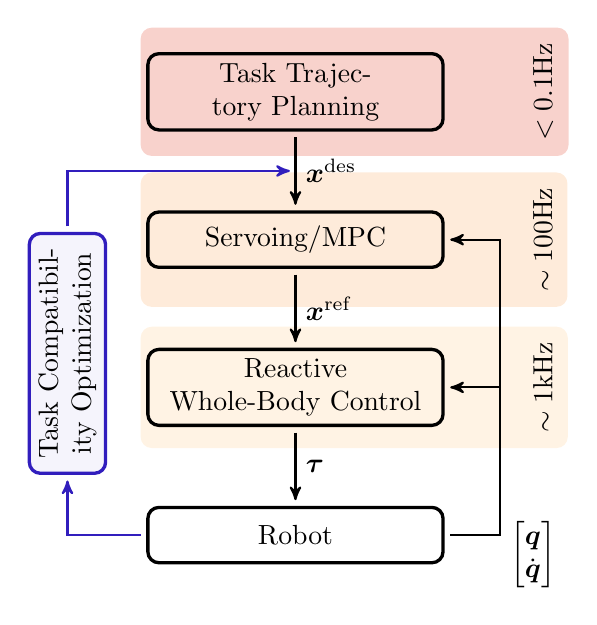
\begin{tikzpicture}[node distance=1cm, auto,]

        \definecolor{planning_color}{RGB}{227,74,51}
        \definecolor{servoing_color}{RGB}{253,187,132}
        \definecolor{wbc_color}{RGB}{254,232,200}

        \node[punkt]                             (planning)  {Task Trajectory Planning};
        \node[punkt, below=1.0cm of planning]       (servoing)  {Servoing/MPC};
        \node[punkt, below=1.0cm of servoing]    (wbc)       {Reactive\\Whole-Body Control};
        \node[punkt, below=1.0cm of wbc]         (robot)     {Robot};

        \node[right=1.0cm of planning] (planning_freq) {\rotatebox{90}{$<0.1$Hz}};
        \node[right=1.0cm of servoing] (servoing_freq) {\rotatebox{90}{$\sim100$Hz}};
        \node[right=1.0cm of wbc] (wbc_freq) {\rotatebox{90}{$\sim1$kHz}};

        \path[pil]
            (planning) edge node [midway, right] {$\x^{\text{des}}$} coordinate [pos=0.5] (top) (servoing)
            (servoing) edge node [midway, right] {$\x^{\text{ref}}$} (wbc)
            (wbc) edge node [midway, right] {$\bs{\tau}$} coordinate [pos=0.5] (bottom) (robot);

        \draw[pil](robot.east) -- ++(20pt,0pt) |- node [midway, right, yshift=-4cm] {$\begin{bmatrix}\q \\ \qd\end{bmatrix}$} (servoing.east) ;
        \draw[pil](robot.east) -- ++(20pt,0pt) |- (wbc.east);

        \node[optim_box, left=1.0cm of servoing, rotate=90, xshift=0.1cm]    (optim)     {Task Compatibility Optimization};

        \draw[optim_pil] (robot.west) -| (optim.west);
        \draw[optim_pil] (optim.east) |- (top);

        \begin{pgfonlayer}{background}
            \node[fill=planning_color!25, rounded corners, inner sep=2pt, fit=(planning)(planning_freq)] {};
            \node[fill=servoing_color!30, rounded corners, inner sep=2pt, fit=(servoing)(servoing_freq)] {};
            \node[fill=wbc_color!50, rounded corners, inner sep=2pt, fit=(wbc)(wbc_freq)] {};
        \end{pgfonlayer}

    \end{tikzpicture}
  	\end{minipage}\hfill
  \begin{minipage}[c]{0.47\textwidth}
      \setlength{\belowcaptionskip}{-12pt}
    \caption{A modern control hierarchy for highly redundant robotic systems, e.g. humanoid robots. At the lowest level is whole-body control, which determines the torques needed to accomplish a set of tasks. At the intermediate level, these tasks are controlled by the servoing/MPC level where task trajectory errors are compensated using state feedback. Finally the task trajectories are provided by high-level planning, which is usually a combination of operator expertise and automated planning. Each of these levels operates independently from one another and a feedback mechanism is needed to measure and compensate for tasks which are not executed as planned. This is the role of the Task Compatibility Optimization loop proposed in this work.}
\label{fig:control_diagram}
  \end{minipage}
\end{figure}

The objective of the proposed approach is to establish the task compatibility optimization loop, shown on the left in Fig.~\ref{fig:control_diagram}, by iteratively improving task trajectories using RL. To do so, some details are provided on how task trajectories are parameterized providing variables with which they can be modified. A generic task compatibility cost is then developed from simple principles which measures the incompatibility between one or more tasks and the robot's constraints. Using two common BBO solvers, this compatibility cost is minimized by optimizing the task trajectory parameters. This task compatibility optimization is then tested on two typical muti-task scenarios. In the first scenario the relatively banal chore of reaching while balancing is studied. While seemingly simple, reaching is a key ingredient in robot autonomy, which often requires parameter and gain tuning before done reliably. A performance comparison of two BBO solvers for this experiment is presented to illustrate the generality of the framework. The second experiment explores the dynamically complex activity of moving from sitting to standing. This motion requires contact breaking and potentially unstable dynamic equilibrium to succeed. In both experiments a Center of Mass (CoM) task is used to maintain balance, and its trajectory is optimized to minimize the task compatibility cost. Through these two completely different motion scenarios, the proposed generic task compatibility optimization loop is shown to dramatically improve task achievement, without ever touching the low-level control parameters.


\section{Methods}
\label{sec:methods}
In this section, the methods and tools used to develop the task compatibility optimization are described. First, trajectory parameterization is detailed. A task compatibility cost is then developed to measure the degree of incompatibility between one or multiple tasks. A brief overview of the two BBO solvers used is provided. Finally the use of these components to optimize task compatibility is explained.

\subsection{Task Parameterization}
\label{sec:task_parameterization}

    For the purpose of brevity, here,  Cartesian acceleration tasks only are considered. In the whole-body controller used in this study, \cite{Salini2011}, an acceleration task error, $T_i$, is formulated as,
    %
    \begin{equation}
         T_{i} = \left\| J_{i}(\q)\qdd + \dot{J}_{i}(\q, \qd)\qd - \xdd^{\text{ref}}_{i} \right\|^2 \tc
        \label{eq:acceleration_task_error}
    \end{equation}
    %
    where $J_{i}$ and $\dot{J}_{i}$, are the task Jacobian and its derivative, $[\q, \qd]$, the \js\ state variable and $\xdd^{\text{ref}}_{i}$ the reference \os\ acceleration. The $\xdd^{\text{ref}}_{i}$ values are provided by task servoing, which are feedforward proportional-derivative controllers. These trajectories are generated from a series of keyframes/waypoints, which represent task coordinates of particular importance. A single position waypoint is given by $\blam_i~=~\x_{i} = \begin{bmatrix} x & y & z \end{bmatrix}^T_i$,
    while a set of $n_{\lambda}$ waypoints is denoted
%
$\Lambda = \begin{bmatrix} \blam_1 & \blam_2 & \dots & \blam_{n} \end{bmatrix}$. Given $\Lambda$, a variety of methods exist for generating a trajectory, e.g. splines, polynomials, optimal control methods, etc. In this study  the time-optimal formulation proposed by \cite{Kunz2012} is used, which can be passed $\Lambda$ and returns a time-optimal trajectory through the waypoints, with a duration, $d_{\Lambda}$, dependent on the velocity and acceleration limits imposed on the movement.

\subsection{Task Compatibility Cost}
\label{sec:task_compatibility_cost}
In this section a measure of task compatibility is derived from simple principles related to the task error objective function in~\eqref{eq:acceleration_task_error}.

    \subsubsection{Tracking Cost}
        In \eqref{eq:acceleration_task_error}, $\xdd^{\text{ref}}_{i}$ is the optimal \os\ value for $T_i$ at time, $t$. If the objective is perfectly realized then the squared norm error is zero, meaning that the robot perfectly follows the task's \os\ reference. Therefore, any error in the position tracking reflects an imperfect optimization of the squared norm task error and consequently a task incompatibility. Using this concept, a \textit{tracking cost} is defined as
        %
        \begin{equation}
        \label{eq:tracking_cost}
        j_{t}^{i} = \displaystyle\sum_{t=0.0}^{t_{\text{end}}} \| \x_{i}(t) - \x_{i}^{\text{ref}}(t) \|^2 \tc
        \end{equation}
        %
        \noindent where $\x_{i}(t)$, is the task frame position and $\x_{i}^{\text{ref}}(t)$, its reference, at time $t$. The term $t_{\text{end}}$ is the actual total duration of the whole-body motion.
        %
    \subsubsection{Goal Cost}
        The assumption is made that the ultimate objective of any point to point trajectory is to reach its target coordinate, or final waypoint. With this in mind a \textit{goal cost} is developed as,
        \begin{equation}
        \label{eq:goal_cost}
        j_{g}^{i} = \displaystyle\sum_{t=0.0}^{t_{\text{end}}} \frac{t}{d_{\Lambda}} \| \x_{i}(t) - \blam_{n} \|^2 \tc
        \end{equation}
        %
        \noindent where $\x_{i}(t) - \blam_{n}$, is the difference between the task's position at $t$ and the final waypoint in its trajectory. The weight of this difference increases linearly from $0.0$ with time.

    \subsubsection{Energy Cost}
        Finally, given the redundancy of the system, it is possible that many whole-body motions exist for the execution of the same set of $n_{\text{tasks}}$ tasks to be performed. To reduce these possibilities, those which are energy optimal are favoured using an \textit{energy cost},
        %
        \begin{equation}
        \label{eq:energy_cost}
        j_{e} = \beta \displaystyle\sum_{t=0.0}^{t_{\text{end}}} \|\bs{\tau}(t) \|^2  \tc
        \end{equation}
        %
        where the term $\beta$ is used to scale the energy cost for meaningful comparison with $j_{t}$ and $j_{g}$. Here, $\beta=1.0\text{e}{-4}$ is used.

    \subsubsection{Compatibility Cost}
        The compatibility cost for $n_{\text{tasks}}$ tasks can be calculated by first summing their tracking and goal costs, then adding the energy cost, which is common to all tasks, and finally averaging over $t_{\text{end}}$,
        %
        \begin{equation}
        \label{eq:total_compatibility_cost}
        j_{c} = \left. \left[ j_{e} + \displaystyle\sum_{i=1}^{n_{\text{tasks}}} \left( j_{t}^{i} + j_{g}^{i} \right) \right] \middle/ t_{\text{end}} \right. \tp
        \end{equation}
        %
        With \eqref{eq:total_compatibility_cost}  the compatibility cost of an arbitrary number of tasks can be estimated. This cost, however, has no absolute significance on its own. There is no threshold value for determining if a set of tasks is compatible, incompatible, or somewhere in between. For any task set, the $j_{c}$ of the initial task trajectories, denoted $j_{c}^{\prime}$, are taken as the reference with which all other task trajectories are compared using,
        %
        \begin{equation}
        \label{eq:scaling_total_compatibility_cost}
        j_{c}^{\text{new}} = \frac{j_{c}}{j_{c}^{\prime}} \tp
        \end{equation}
        %
        This means that for any task combination, the initial task trajectories have a compatibility cost equal to $1.0$. Any modifications to the trajectories yielding a $j_{c}^{\text{new}} < 1.0$ represent improvements in task compatibility, and vice versa for $j_{c}^{\text{new}} > 1.0$.\\

        Finally  tasks  used for computation of \eqref{eq:total_compatibility_cost} must be determined. In a typical whole-body controller there may be a multitude of simultaneously active tasks at any given time. Generally there are a few primary tasks which are designed to affect some motion, and any number of helper tasks used to improve the stability, posture, or quality of the movement. The decision of which tasks to use to calculate \eqref{eq:total_compatibility_cost} is an open one, but here the principal tasks are used, such as those for balance and reaching.


\subsection{BBO Solvers}
\label{sec:bbo_solvers}
The task compatibility optimization problem is non-linear, non-convex, and possibly discontinuous. BBO solvers are therefore used. Local solvers, such as Covariance Matrix Adaptation Evolutionary Strategy (CMA-ES) use the statistics from a set of objective variable samples and their costs to estimate the mean and covariance of the sample distribution and then update this distribution in the direction of the natural gradient \cite{Ollivier2011}. Global solvers such as Bayesian Optimization (BO) explicitly model the latent cost function using Gaussian Processes and provide a set of parameters to test which both minimize the expected cost and the uncertainty of the cost model \cite{Rasmussen2006}.\\
%
%
%   Note to self... Adding the acknowledgements makes the paper too long and I can't seem to fix it with tricks. So I removed the Cully2015 reference which was the least related to robotic control in this context. In the camera ready try to add it back in by editing the text to be more concise.
%
%
% BO solvers usually require fewer trials to obtain an optimal solution and have become a popular choice in robotics because of this efficiency \cite{Calandra2014, Antonova2016, Cully2015, Englert2016}.
BO solvers usually require fewer trials to obtain an optimal solution and have become a popular choice in robotics because of this efficiency \cite{Calandra2014, Antonova2016, Englert2016}.
The performance and solution quality of BO and CMA-ES are highly dependent on proper tuning of the solver meta-parameters; e.g. kernel type, kernel parameters, acquisition function, initial variance, etc. To properly compare solvers, meta-parameters for BO and CMA-ES are selected to ensure consistent convergence without being overly greedy, and are maintained for all experiments.
%


\subsection{Task Compatibility Optimization}
\label{sec:task_compatibility_optimization}
\begin{algorithm}[!h]
    \caption{Task Compatibility Optimization}
    \label{algo:task_compatibility_optimization}
    \begin{algorithmic}[1]
        \State Given a set of tasks to execute on a whole-body controller.
        \State Select task waypoint to be optimized: $\obj_{\text{new}} = \blam_{i}$.
        \State $\Obj = [\ ]$ and $\bs{j} = [\ ]$.
        \Do
            \State Generate task trajectory with $\blam_{i} = \obj_{\text{new}}$.
            \State Simulate task set execution.
            \State Compute $j_{c}$ with \eqref{eq:total_compatibility_cost}.
            \If{first iteration}
                \State $j_{c}^{\prime} = j_{c}$
            \EndIf
            \State Calculate $j_{c}^{\text{new}} = \frac{j_{c}}{j_{c}^{\prime}}$.
            \State $\Obj = \left[\Obj, \obj_{\text{new}} \right]$
            \State $\bs{j} = \left[\bs{j}, j_{c}^{\text{new}} \right]$
            \State Update solver with $\Obj$ and $\bs{j}$.
            \State Get new waypoint to test $\obj_{\text{new}}$.
        \doWhile{\eqref{eq:convergence_criterion} is false}
        \State\Return $\obj_{\text{best}}$
    \end{algorithmic}
\end{algorithm}

    In this section, the algorithm for optimizing task compatibility is developed. A set of tasks with various priorities and gains that are fixed is assumed to be given. Initial trajectories for these tasks are provided by a human operator manually selecting waypoints. Given the task parameterization described in Section \ref{sec:task_parameterization}, one or more task waypoints can be used as the objective variable, $\obj$. By modifying these waypoints, the resulting task trajectory is modified and consequently, the overall whole-body behavior. The first step in the optimization is then to select the waypoint(s) which serve as the objective variable. Here, the use of one waypoint only is considered so the objective variable is simply $\obj = \blam_{i}$. The cost associated with $\obj$ is then evaluated using \eqref{eq:total_compatibility_cost} after simulating the execution of the tasks. The simulation is stopped when either all tasks have been completed or a fixed amount of time has elapsed. This initial compatibility cost is used as the baseline, $j_{c}^{\prime}$, to which all subsequent costs are compared. The observed parameter and cost samples are concatenated together into $\Obj$ and $\bs{j}$, respectively, and provided to either BO or CMA-ES.
    The solver proposes a new objective variable to test, $\obj_{\text{new}}$ to use as the task waypoint and the task trajectory is regenerated. The task set is then executed and its compatibility cost, $j_{c}^{\text{new}}$, is calculated. Both $\obj_{\text{new}}$ and $j_{c}^{\text{new}}$ are concatenated to the current objective variable-cost pairs, and the solver is updated again. This process is iterated until,
        %
        \begin{equation}
            \left\| \obj_{\text{new}} - \obj_{\text{best}} \right\| \leq \Psi \tc
            \label{eq:convergence_criterion}
        \end{equation}
        %
        where $\obj_{\text{best}}$ is the best observed waypoint with the lowest cost and $\Psi$ is a meta-parameter which dictates the minimum threshold for convergence. When converged, the algorithm returns the optimal waypoint, $\obj_{\text{best}}$, with the best observed compatibility cost. This is detailed in Algorithm \ref{algo:task_compatibility_optimization}.

\begin{figure}[!h]
	\begin{minipage}[c]{0.6\textwidth}
	\centering
    \subfloat[] {
        \includegraphics[height=4.2cm, trim={6cm 16cm 8cm 18cm}, clip]{reaching/reaching_targets}
        \label{fig:reaching_targets}
    }
    \subfloat[] {
        \includegraphics[height=4.2cm, trim={5cm 5cm 5cm 6cm}, clip]{reaching/reaching_com_bounds}
        \label{fig:reaching_com_bounds}
    }
    \subfloat[] {
        \includegraphics[height=4.2cm, trim={10cm 14cm 2cm 4.5cm}, clip]{standing/standing_com_bounds}
        \label{fig:standing_com_bounds}
    }
  	\end{minipage}\hfill
  \begin{minipage}[c]{0.37\textwidth}
      \setlength{\belowcaptionskip}{-12pt}
    \caption{Figure \protect\subref{fig:reaching_targets} shows the random reaching targets used to provide a statistical analysis of the task compatibility optimization described in Section \ref{sec:methods}. The target spheres are color coded to indicate their test case, with green meaning reachable, orange meaning possibly reachable, and red meaning unreachable. These test cases are detailed in Section \ref{sec:experiments_reaching}. Figures \protect\subref{fig:reaching_com_bounds} and \protect\subref{fig:standing_com_bounds} show the $\obj_{\text{new}}$ bounding boxes used for the task compatibility optimization of the reaching and standing experiments, respectively.}
    \label{fig:experiments_figures}
  \end{minipage}
\end{figure}

\begin{figure*}[!t]
    \centering
    \vspace{0.2cm}
        \begin{minipage}{0.32\linewidth}
            \centering
            reachable

            \subfloat[] {
                \includegraphics[
                    height=4.5cm,
                    width=.45\textwidth,
                    keepaspectratio,
                    trim={12cm 3cm 6cm 4cm},
                    clip]
                    {reaching/reachable_original}
                \label{fig:reachable_case_original}
            }
            \hfil
            \subfloat[] {
                \includegraphics[
                    height=4.5cm,
                    width=.45\textwidth,
                    keepaspectratio,
                    trim={12cm 3cm 6cm 4cm},
                    clip]
                    {reaching/reachable_optimal}
                \label{fig:reachable_case_optimal}
            }

            \subfloat[] {
                \includegraphics[width=1.0\textwidth]{reaching/reachable_case_statistics}
                \label{fig:reachable_case_statistics}
            }

        \end{minipage}
        \hfil
        \begin{minipage}{0.32\linewidth}
            \centering
            possibly reachable

            \subfloat[] {
                \includegraphics[
                    height=4.5cm,
                    width=.45\textwidth,
                    keepaspectratio,
                    trim={13cm 3cm 0cm 4cm},
                    clip]
                    {reaching/possibly_reachable_original}
                \label{fig:possibly_reachable_case_original}
            }
            \hfil
            \subfloat[] {
                \includegraphics[
                    height=4.5cm,
                    width=.45\textwidth,
                    keepaspectratio,
                    trim={13cm 3cm 0cm 4cm},
                    clip]
                    {reaching/possibly_reachable_optimal}
                \label{fig:possibly_reachable_case_optimal}
            }

            \subfloat[] {
                \includegraphics[width=1.0\textwidth]{reaching/possibly_reachable_case_statistics}
                \label{fig:possibly_reachable_case_statistics}
            }
        \end{minipage}
        \hfil
        \begin{minipage}{0.32\linewidth}
            \centering
            unreachable


            \subfloat[] {
                \includegraphics[
                    height=4.5cm,
                    width=.45\textwidth,
                    keepaspectratio,
                    trim={11cm 3cm 0cm 4cm},
                    clip]
                    {reaching/unreachable_original}
                \label{fig:unreachable_case_original}
            }
            \hfil
            \subfloat[] {
                \includegraphics[
                    height=4.5cm,
                    width=.45\textwidth,
                    keepaspectratio,
                    trim={11cm 3cm 0cm 4cm},
                    clip]
                    {reaching/unreachable_optimal}
                \label{fig:unreachable_case_optimal}
            }


            \subfloat[] {
                \includegraphics[width=1.0\textwidth]{reaching/unreachable_case_statistics}
                \label{fig:unreachable_case_statistics}
            }
        \end{minipage}


        \setlength{\belowcaptionskip}{-10pt}
        \caption{Results of $100$ reaching experiments used to study the task compatibility optimization method. An average example is presented for the three possible reach cases.
        In the reachable case, \protect\subref{fig:reachable_case_original} \& \protect\subref{fig:reachable_case_optimal}, both the original and optimized movements attain the reach target.
        In the possibly reachable case, \protect\subref{fig:possibly_reachable_case_original} \& \protect\subref{fig:possibly_reachable_case_optimal}, the original movement does not attain the target but the optimized movement does.
        Finally in the unreachable case, \protect\subref{fig:unreachable_case_original} \& \protect\subref{fig:unreachable_case_optimal}, neither movement attains the target, but the optimized movement reduces the target error.
        For each case, the relative cost means and standard deviations are plotted for both the BO and CMA-ES solvers. Any relative cost lower than $1.0$ is an improvement (the $1.0$ line is indicated by a dashed grey lines).
        For all three cases the relative compatibility cost $j_{c}^{\text{best}}$ is always less than or equal to $1.0$. This indicates that the optimized movements will always be as good if not better than the original movements.
        In the reachable case, \protect\subref{fig:reachable_case_statistics}, little improvement is seen because the tasks are already compatible.
        For the possibly reachable and unreachable cases, \protect\subref{fig:possibly_reachable_case_statistics} and \protect\subref{fig:unreachable_case_statistics}, the compatibility is improved by reducing the tracking and goal costs at the expense of increased energy usage.
        For each of the cases BO outperformed CMA-ES in convergence iterations on average, but was less consistent across-the-board. See Section \ref{sec:results_reaching} for more details.}
        \label{fig:reaching_case_examples}
    \end{figure*}


\section{Experiments}
\label{sec:experiments}

The experiments presented in this section are designed to illustrate the task compatibility optimization described in Section \ref{sec:methods}, compare the performances of BBO solvers used within the method, and highlight the subtle complexities of common tasks from the perspective of whole-body control. A simulation of a humanoid robot, iCub, is used for these studies. Gazebo is used as the simulation environment with the ODE physics engine.\\

The first experiment explores basic \textit{reaching} movements under bipedal equilibrium, and serves as a benchmark for the task compatibility optimization method. It provides us with useful statistics to analyze the method and BBO solvers. The second experiment, entitled \textit{standing} presents a more dynamically complex scenario in which the robot starts from a seated position and must transition to standing. Here, the difficulties of contact transitioning and dynamic equilibrium is studied. In both experiments, balance is achieved by keeping the robot's CoM position over its Polygon of Support (PoS). The PoS is defined by the convex hull of the active model contacts in the whole-body controller.\\

Each experiment begins with a fixed set of tasks, parameters and gains. In the following, right hand and CoM tasks only are discussed, but it should be noted that postural, torso orientation, and left hand tasks are also active during the motion. The tasks all have initial trajectories which are generated from waypoints, picked by an expert operator. For both reaching and standing the CoM task trajectory is optimized to improve the task compatibility cost. Box constraints for the optimization can be applied in both BO and CMA-ES and are set here using static stability constraints, i.e. the projection of the CoM must remain inside the PoS. The $z$ bounds are chosen as $0.3\text{m} \leq z \leq 0.52\text{m}$. The bounding boxes for both experiments are shown in Figs.~\ref{fig:reaching_com_bounds} and \ref{fig:standing_com_bounds}.\\

All code for these experiments is open-source and can be found here: {\small \url{https://github.com/rlober/ra-l_2017.git}}.




\subsection{Reaching}
\label{sec:experiments_reaching}


    This experiment is concerned with demonstrating the flexibility of the proposed task compatibility optimization, as well as gleaning useful statistics about the two proposed solvers, BO and CMA-ES. To accomplish this, $100$ reach targets are randomly generated around the simulated robot, see Fig.~\ref{fig:reaching_targets}. For each target, a straight line trajectory is generated for the right hand task between its starting position and the target's position. The CoM task trajectory is generated between two waypoints,
    %
    \begin{equation}
        \Lambda_{\text{CoM}} = \begin{bmatrix} \lambda_{\text{start}} & \lambda_{\text{goal}} \end{bmatrix} \tc
        \label{eq:com_reaching_waypoints}
    \end{equation}
    %
    where $\lambda_{\text{start}}$ is the initial CoM position, and $\lambda_{\text{goal}}$ is the desired goal CoM position, which is initially chosen to be the center of the PoS at the current CoM $z$ height. $\lambda_{\text{goal}}$ is chosen as the task compatibility objective variable, $\obj_{\text{new}}$. By optimizing $\lambda_{\text{goal}}$ the CoM trajectory is modified. The compatibility cost, \eqref{eq:total_compatibility_cost}, is computed using right hand and CoM tasks.\\


    The objective of the experiment is to attain the reach target and a target is considered attained when the right hand task frame is within $3.0$cm of it. The movement is stopped if the target is attained or if a time limit is exceeded. For each reach target, the optimization is run using both BO and CMA-ES as solvers. The target is then classified into one of three cases. If the robot attains the target with the original CoM trajectory, the target is considered \textbf{reachable}. If it is unable to attain the target with the original CoM trajectory, but attains the target with the optimized CoM trajectory then the target is \textbf{possibly reachable}. Finally, if the reach target is unattainable with either the original or optimized CoM trajectories, then it is considered \textbf{unreachable}.


\subsection{Standing}
\label{sec:experiments_standing}


    In this experiment, the robot is seated on a stationary bench and the objective is to stand up. In this case the only primary task is the CoM task, and its trajectory is defined by three waypoints,
    %
    \begin{equation}
        \Lambda_{\text{CoM}} = \begin{bmatrix} \lambda_{\text{start}} & \lambda_{\text{middle}} & \lambda_{\text{goal}} \end{bmatrix} \tc
        \label{eq:com_standing_waypoints}
    \end{equation}
    %
    where $\lambda_{\text{start}}$ and $\lambda_{\text{goal}}$ have the same meaning as in \eqref{eq:com_reaching_waypoints} and $\lambda_{\text{middle}}$ is a middle waypoint between the start and goal CoM positions. Here, $\lambda_{\text{goal}}$ is picked as a nominal standing CoM position near the middle of the PoS in $x$ and $y$ and at approximately $0.5$m from the ground,
    and $\lambda_{\text{middle}}$ is picked as a point halfway between $\lambda_{\text{start}}$ and $\lambda_{\text{goal}}$. In this experiment, $\lambda_{\text{middle}}$ is chosen as $\obj_{\text{new}}$.\\
    % , and is bounded by the largest solid box formed by the feet and seat contacts, as shown in Fig.~\ref{fig:standing_com_bounds}. The $z$-height of the bounding box is limited by the maximum standing CoM height, $0.52$m.

    In order to stand, the bench contacts used in the whole-body controller model must be deactivated or the robot will never be able to get up. The bench contacts are deactivated arbitrarily at $2.0$ seconds. The motion is executed until the CoM task has attained $\lambda_{\text{goal}}$ or some time limit has been exceeded. The compatibility cost, \eqref{eq:total_compatibility_cost}, is computed using only the CoM task.







    \begin{figure}[!h]
        \centering
        \subfloat[original\label{fig:standing_original}] {
            \setlength\tabcolsep{0pt}
            \begin{tabular}{cccc}
                \includegraphics[
                width=0.25\columnwidth,
                height=6cm,
                keepaspectratio,
                trim={12cm 25cm 12cm 22cm},
                clip]{standing/standing_original_0} &
                \begin{overpic}[
                width=0.25\columnwidth,
                height=6cm,
                keepaspectratio,
                trim={5cm 9cm 0cm 0cm},
                clip]{standing/standing_original_1}
                \put(35,90) {$2.0$s}
                \end{overpic} &
                \begin{overpic}[
                width=0.25\columnwidth,
                height=6cm,
                keepaspectratio,
                trim={5cm 9cm 0cm 0cm},
                clip]{standing/standing_original_2}
                \put(35,90) {$2.5$s}
                \end{overpic} &
                \begin{overpic}[
                width=0.25\columnwidth,
                height=6cm,
                keepaspectratio,
                trim={5cm 9cm 0cm 0cm},
                clip]{standing/standing_original_3}
                \put(35,90) {$3.0$s}
                \end{overpic}
            \end{tabular}
        }

        \subfloat[optimized\label{fig:standing_optimized}] {
            \setlength\tabcolsep{0pt}
            \begin{tabular}{cccc}
                \includegraphics[
                width=0.25\columnwidth,
                height=6cm,
                keepaspectratio,
                trim={12cm 25cm 12cm 22cm},
                clip]{standing/standing_optimized_0} &
                \begin{overpic}[
                width=0.25\columnwidth,
                height=6cm,
                keepaspectratio,
                trim={5cm 9cm 0cm 0cm},
                clip]{standing/standing_optimized_1}
                \put(35,90) {$2.0$s}
                \end{overpic} &
                \begin{overpic}[
                width=0.25\columnwidth,
                height=6cm,
                keepaspectratio,
                trim={5cm 9cm 0cm 0cm},
                clip]{standing/standing_optimized_2}
                \put(35,90) {$4.0$s}
                \end{overpic} &
                \begin{overpic}[
                width=0.25\columnwidth,
                height=6cm,
                keepaspectratio,
                trim={5cm 9cm 0cm 0cm},
                clip]{standing/standing_optimized_3}
                \put(35,90) {$5.0$s}
                \end{overpic}
            \end{tabular}
        }
        \setlength{\belowcaptionskip}{-10pt}
        \caption{Original and optimized CoM reference trajectories and their resultant whole-body motions. The original trajectory produces an unstable standing motion causing the robot to lose balance. The optimized CoM trajectory, however, produces a successful sit-to-stand transition. The right hip is translucent in \protect\subref{fig:standing_optimized} to make the reference trajectory visible.}
        \label{fig:standing_images}
    \end{figure}

%\addtolength{\textheight}{-0.3cm}   % This command serves to balance the column lengths
                                  % on the last page of the document manually. It shortens
                                  % the textheight of the last page by a suitable amount.
                                  % This command does not take effect until the next page
                                  % so it should come on the page before the last. Make
                                  % sure that you do not shorten the textheight too much.
\section{Results}
\label{sec:results}

In this section the results for the reaching and standing experiments are presented. Please see the accompanying video for a better look at the results presented here.

\subsection{Reaching}
\label{sec:results_reaching}

    In Fig.~\ref{fig:reaching_case_examples} shows representative examples of the three reach cases. For each, the relative cost means and optimization iteration means are computed. The relative compatibility cost, $j_{c}^{\text{best}}$, and the component relative costs, $j_{e}^{\text{best}}$, $j_{g}^{\text{best}}$, and $j_{t}^{\text{best}}$, are calculated by dividing the optimized costs by the original costs.\\

    In the reachable case, Figs.~\ref{fig:reachable_case_original}, \ref{fig:reachable_case_optimal} and \ref{fig:reachable_case_statistics}, it can be seen that the original task trajectories go unmodified because they are already compatible. In a few cases CMA-ES is able to improve slightly on the compatibility cost.
   Compatibility cost improvements can be observed between $30\%$-$50\%$ in the possibly reachable case, Figs.~\ref{fig:possibly_reachable_case_original}, \ref{fig:possibly_reachable_case_optimal} and \ref{fig:possibly_reachable_case_statistics}, where both solvers quickly converge on solutions which reduce the tracking and goal errors allowing the robot to attain the reach target. These improvements require increased energy usage to move the CoM, but the resulting successful reach which finishes more quickly, amortizing the impact of the increased energy cost.
    In the unreachable case, Figs.~\ref{fig:unreachable_case_original}, \ref{fig:unreachable_case_optimal} and \ref{fig:unreachable_case_statistics}, cost improvements similar to those in the possibly reachable case can be seen, despite the fact that the targets are physically unattainable.\\

    For all three cases, BO and CMA-ES show similar performance in terms of cost reduction. In terms of convergence iterations, BO tends to find an optimum in approximately half the number of iterations needed by CMA-ES, however is less consistent than CMA-ES across-the-board.

\subsection{Standing}
\label{sec:results_standing}


\begin{figure}[!h]
	\begin{minipage}[c]{0.6\textwidth}
	\centering
    \includegraphics[width=\textwidth, trim={0cm 0.5cm 0cm 0cm}, clip]{standing/standing_traj}
  	\end{minipage}\hfill
  \begin{minipage}[c]{0.37\textwidth}
	\setlength{\belowcaptionskip}{-10pt}
    \caption{Evolution of the CoM for the original and optimized movements. The original CoM curves are cut off after $2.7$ seconds when the robot loses balance. The red dashed line indicates the moment when the bench contacts are deactivated in the whole-body controller.}
    \label{fig:standing_traj}
  \end{minipage}
\end{figure}

In Fig.~\ref{fig:standing_images},  the evolution the CoM for the original and optimized movements is provided. The whole-body motion produced by the original CoM trajectory, Fig.~\ref{fig:standing_original}, is unstable and causes the robot to loose balance. The optimized CoM trajectory, on the other hand, produces a stable sit-to-stand transition as shown in Fig.~\ref{fig:standing_optimized}. In Fig.~\ref{fig:standing_traj} it is observed that, at the moment the bench contacts are deactivated in the controller (the dashed vertical red line), the original motion immediately tends to lift the CoM upwards, despite an inappropriate $x$-location of the CoM (not close enough to the foot PoS). This inconsistent CoM trajectory does not respect the dynamic balancing conditions (see \cite{Perrin2015}) and causes the robot to fall.%A detailed analysis of the loss of balance is beyond the scope of this paper.
The optimized trajectory moves the CoM more aggressively in the forward direction as well as lowering it prior to the contact deactivation instant. The resulting CoM trajectory is balance consistent, thus leading to a successful sit-to-stand transition.\\

A video associated to these results and submitted with~\underline{\bf \cite{lober2017RAL-IROS}} can be viewed here: \url{https://tinyurl.com/hszx2qs}.

\subsection{Towards year 4 demonstration}

 \begin{figure}[!h]
        \centering
           \setlength\tabcolsep{0pt}
            \begin{tabular}{cccc}
               \begin{overpic}[
                width=0.25\textwidth,
%                height=6cm,
%                keepaspectratio,
%                trim={12cm 25cm 12cm 22cm},
                clip]{with_forces/standing_traj_original}
                \put(10,90) {\bf Original}
                \end{overpic} &
                \begin{overpic}[
                width=0.25\textwidth,
%                height=6cm,
%                keepaspectratio,
%                trim={5cm 9cm 0cm 0cm},
                clip]{with_forces/standing_traj_optimized}
                \put(10,90) {\bf Optimized}
                \end{overpic} &
                \begin{overpic}[
                width=0.25\textwidth,
%                height=6cm,
%                keepaspectratio,
%                trim={5cm 9cm 0cm 0cm},
                clip]{with_forces/standing_traj_original_with_force}
                \put(0,90) {\bf Original w/ force}
                \end{overpic} &
                \begin{overpic}[
                width=0.25\textwidth,
%                height=6cm,
%                keepaspectratio,
%                trim={5cm 9cm 0cm 0cm},
                clip]{with_forces/standing_traj_optimized_with_force}
               \put(0,90) {\bf Optimized w/ force}
                \end{overpic}
            \end{tabular}
        \setlength{\abovecaptionskip}{-20pt}
        \caption{Original and optimized CoM reference trajectories. The original trajectory produces an unstable standing motion causing the robot to lose balance. The optimized without support and externally supported cases produce successful sit-to-stand transitions.}
        \label{fig:standing_images_with_forces}
    \end{figure}

In preparation of the final year demonstration, the CoM task optimization for standing is also tested in simulations including external support. Here external support is simulated, in simple and naive way, as an external force applied at each forearm of the robot through out the overall movement. The magnitude of the force at each forearm is chosen small: $F_{support} = 5.23~N$ pointing $45^{\circ}$ upward and front in the sagittal plane of the robot. Including the two aforementioned ``original'' and ``optimized movement'', two extra cases are tested:  original movement with external support and optimized movement with external support. The resulting CoM trajectories are presented in Fig.~\ref{fig:standing_images_with_forces}.\\

The results in terms of compatibility cost optimization are presented in Fig.~\ref{fig:standing_w_forces_costs}. As intuitively expected, the use of an external supporting force together with an optimized CoM trajectory yields the best results in terms of tracking and whole-body energy expenditure. The main difference between the optimized motion without external support and the optimized motion with external support lies in the energetic expenditure and time needed to reach a standing posture. This is also illustrated in Fig.~\ref{fig:standing_traj_with_forces} where the time needed to reach the CoMheight $z_{COM} = 0.5~m$ is more than $1.5\times$ larger (measured from the instant where bench contact constraints are no longer enforced) in the case where no external support is present.

\begin{figure}[!h]
	\begin{minipage}[c]{0.6\textwidth}
	\centering
    \includegraphics[width=\textwidth, trim={0cm 0.5cm 0cm 0cm}, clip]{with_forces/standing_costs}
  	\end{minipage}\hfill
  \begin{minipage}[c]{0.37\textwidth}
      \setlength{\belowcaptionskip}{-12pt}
    \caption{The costs presented here corresponds to the three following cases: optimized movement without external support, original movement with external support and optimized movement with external support. Each cost is presented as a ratio of the original cost (no optimization, no external support). As intuitively expected, the use of an external supporting force together with an optimized CoM trajectory yields the best results in terms of tracking and whole-body energy expenditure.}
    \label{fig:standing_w_forces_costs}
  \end{minipage}
\end{figure}


\begin{figure}[!h]
	\begin{minipage}[c]{0.6\textwidth}
	\centering
   \includegraphics[width=1\textwidth, trim={0cm 0.5cm 0cm 0cm}, clip]{with_forces/standing_trajectories}
  	\end{minipage}\hfill
  \begin{minipage}[c]{0.37\textwidth}
	\setlength{\belowcaptionskip}{-10pt}
    \caption{Evolution of the CoM for the original and optimized movements, without and with support. The original CoM curves without support are cut off after $2.7$ seconds when the robot loses balance. The red dashed line indicates the moment when the bench contacts are deactivated in the whole-body controller.}
    \label{fig:standing_traj_with_forces}
  \end{minipage}
\end{figure}

\section{Conclusion}
    The primary conclusion to draw from this work is that through task compatibility optimization,  the overall performance of a wide variety of movements can be improved using  generic principles. By improve, it is meant that the original intent of the planned task trajectories is better realized. In the reaching experiments this means more targets are attained, and in the standing case it means the robot can successfully transition from sitting to standing. Moreover, the need for fine tuning of controller priorities and gains is alleviated because they are accounted for in the task optimization. In addition, the compatibility optimization concept is controller independent and, while it is expected that the controller described in section~\ref{sec:controller} will be used during the final year demo, the use of another controller would not imply any modification at the task compatibility optimization level.\\
    
     With regards to BBO solvers, a comparison of the BO and CMA-ES reveals that BO tends to converge to an optimal solution in half the number of simulation iterations needed by CMA-ES. Such efficiency is desirable if the optimization iterations are to occur on a real robot.\\

%    The next step in this work is to develop a mathematical model of task compatibility in the context of multi-objective optimization for robotic control. Such a model would open up the possibility of model-based RL, and potentially even more efficient task compatibility optimization.% Another short term perspective is implementation of the standing experiment on the real robot.

    Finally, it is believed that the proposed task compatibility optimization loop is an important first step towards an intermediate control layer between high-level planning and low-level control, where task trajectories are optimized for compatibility before being executed on the real robot, as illustrated by Fig.~\ref{fig:experiment} for a reaching motion. The combination of state-of-the-art whole-body control and task level optimization will hopefully also be  demonstrated during the final year demonstration. Improved results can even be expected using the estimation of the supporting wrenches applied by the caregiver developed in Deliverable~5.4~\cite{deliverable54}.

\begin{figure}[!h]
    \centering
    \subfloat[original\label{fig:experiment_original}] {
        \includegraphics[
            % height=4.5cm,
            width=.36\textwidth,
            keepaspectratio,
            trim={5cm 3cm 0cm 8cm},
            clip
            ]
            {reaching/experiment_original}
    }
    \hfil
    \subfloat[optimized\label{fig:experiment_optimized}] {
        \includegraphics[
            % height=4.5cm,
            width=.36\textwidth,
            keepaspectratio,
            trim={5cm 3cm 0cm 8cm},
            clip
            ]
            {reaching/experiment_optimized}
    }
    \setlength{\belowcaptionskip}{-12pt}
    \caption{An original and optimized reaching motion executed on an iCub robot is illustrated here. These preliminary results show that the movements produced by task compatibility optimization may be viable on real platforms.}
    \label{fig:experiment}
\end{figure}





\newpage{}

\phantomsection
\bibliographystyle{IEEEtran}
% argument is your BibTeX string definitions and bibliography database(s)
\bibliography{IEEEabrv,D3.3,D3.2}
\addcontentsline{toc}{section}{References}




\end{document}

%%% Local Variables:
%%% mode: latex
%%% TeX-master: t
%%% save-place: t
%%% End:
